\defChapterTarget{Esecuzione e Risulati}
    Ogni esaminatore ha assegnato un voto per le singole euristiche prese in
    considerazione. I risultati presenti nelle tabelle presentate in questo
    documento sono ottenuti dalle medie dei valori proposti e sono giustificati
    con motivazioni condivise dagli esaminatori. Di seguito è possibile trovare un grafico 
    con le medie dei voti dei valutatori per ogni euristica.
    \begin{figure}[H]
        \centering
        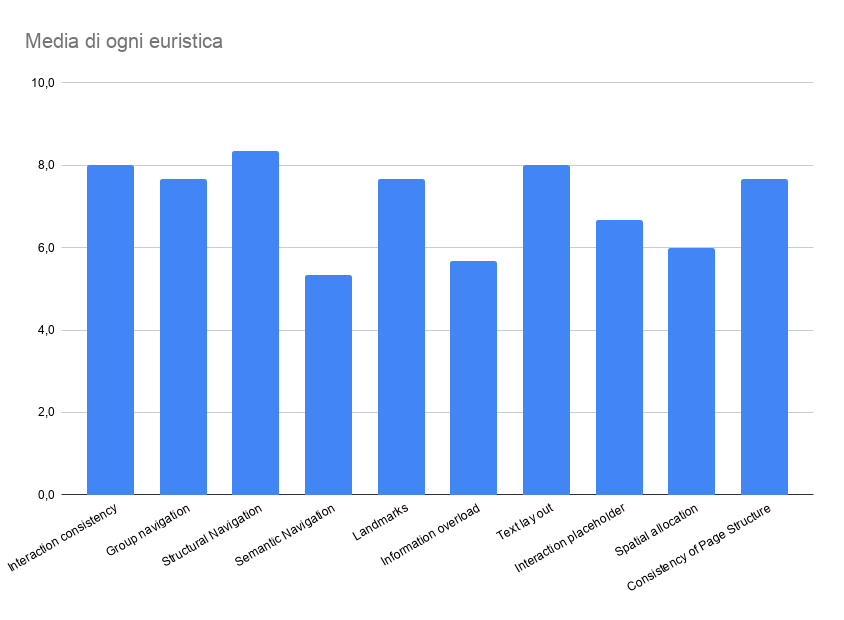
\includegraphics[scale=0.3]{resources/images/graficoMedieEuristiche.png}
    \end{figure}
    \section{Navigazione}
        \begin{table}[H]
        \begin{tabular}{|l|l|l|l|l|}
            \hline \textbf{Euristica} & \textbf{Davide} & \textbf{Marco} &
            \textbf{Fabrizio} & \textbf{Voto totale} \\ \hline
            Consistenza nelle interazioni           & 9.0   & 8.0   & 7.0   & 8.0 \\ \hline
            Navigazione dei gruppi                  & 8.0   & 8.0   & 7.0   & 7.7 \\ \hline
            Navigazione strutturale                 & 10.0  & 7.0   & 8.0   & 8.3 \\ \hline
            Navigazione semantica                   & 5.0   & 6.0   & 5.0   & 5.3 \\ \hline
            Landmarks                               & 9.0   & 6.0   & 8.0   & 7.7 \\ \hline
                                                    &       &       &       & 7.4 \\ \hline
            \end{tabular}
        \end{table}

        \subsection{Consistenza nelle interazioni}
        Le pagine dello stesso tipo hanno generalmente gli stessi links e la
        stessa capacità di interazione. \\
        Ad esempio le pagine Monterosa Ski e Monterosa Discover sono dello
        stesso tipo in quanto risultano entrambe delle pagine principali e sono
        strutturate nello stesso modo per quanto riguarda le tipologie di link e
        capacità interattive. Non sempre questa euristica è rispettata in tutti gli
        elementi, ad esempio nella pagina "Monterosa Kids" non sono presenti i
        links riguardo le nuove proposte che sono invece presenti in Monterosa
        Nature\&Culture.
    
        \subsection{Navigazione dei gruppi}
        La possibilità di spostarsi all’ interno di elementi appartenenti allo
        stesso gruppo è generalmente garantita dalla presenza dei subitems
        presenti nei landmark. \\
        La possibilità di spostarsi da un elemento ad un altro dello stesso
        gruppo è solo in alcuni casi possibile: ad esempio entrando nella pagina
        relativa agli appartamenti è sempre possibile sceglierne un'altra
        tipologia usando la voce tipo di struttura a destra mentre in altri casi
        è necessario dover selezionare nuovamente il gruppo intero come nella sezione
        Monterosa ski, dove il menu a destra non permette di vedere i links relativi 
        agli impianti sciistici.
        \begin{figure}[H]
            \centering
            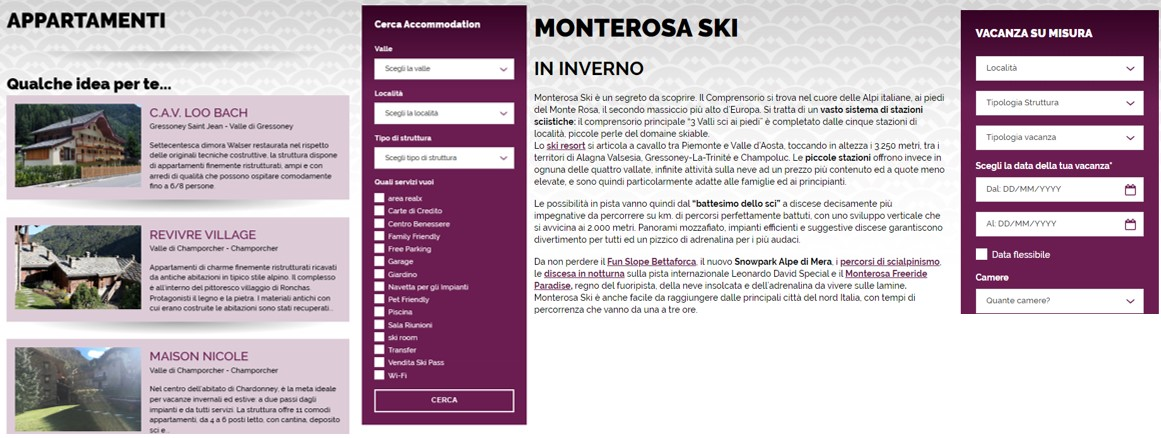
\includegraphics[scale=0.6]{resources/images/groupNavigationFinals.jpg}
        \end{figure}

        \subsection{Navigazione strutturale}
        Il sito rende possibile l'esplorazione di ogni pagina partendo dai link
        presenti all’interno del corpo. Un esempio è  la pagina principale
        Discover Monterosa. Un altro esempio che possiamo considerare è la
        pagina Monterosa Active, dove i singoli link  (sci alpinismo, sci di
        fondo, ice climbing, ciaspole, sci, heliski) sono chiaramente
        evidenziati nella pagina. Questi link sono inoltre raggiungibili anche
        dal menu in testa al sito rendendo ancora più veloce la navigazion verso
        l’elemento di interesse. Tutto questo consente alla pagina Monterosa
        Active di non avere troppe informazioni al suo interno, dividendo il suo
        contenuto nelle altre pagine dedicate ai singoli elementi. Non sempre la
        suddivione dei subitem nei menu è intuitiva. Ad esempio la categoria
        "Monterosa Ski" presenta troppi elementi pochi chiari.

        \subsection{Navigazione semantica}
        Ogni tanto non è facile muoversi tra argomenti che hanno degli elementi
        in comune, ad esempio il link "Maestri di sci" è presente solo nella
        homepage, ma ci si aspetterebbe di trovarlo anche come sub-item del menu
        "Monterosa Ski". \\ Un elemento che risulta poco chiaro e in un
        certo senso anche “oppressivo” è l’onnipresenza del menu di
        prenotazione della vacanza sul lato destro delle pagine, presente anche
        in pagine che non dovrebbero averlo.
        Un elemento positivo è dato dalla presenza dei link
        "Potrebbe interessarti" che permettono di raggiungere velocemente
        informazioni correlate.

        \subsection{Landmarks}
        I Landmarks sono molto utili per spostarsi all'interno del sito ed in
        particolar modo risultano essere importanti per tornare indietro nel
        caso si fosse entrati nella sezione sbagliata. 
        La presenza ulteriore di shortcuts all’ interno della pagina risulta
        essere un po’ eccessiva in quanto i collegamenti sono già individuabili
        all'interno dei “landmarks” presenti in alto nella pagina.
  
    \section{Contenuto}
    \begin{table}[H]
        \begin{tabular}{|l|l|l|l|l|}
        \hline \textbf{Euristica} & \textbf{Davide} & \textbf{Marco} &
        \textbf{Fabrizio} & \textbf{Voto totale} \\ \hline
        Sovraccarico di informazioni    & 7.0   & 6.0   & 4.0   & 5.7 \\ \hline
                                        &       &       &       & 5.7 \\ \hline
        \end{tabular}
        \end{table}
        \subsection{Sovraccarico di informazioni}
        Le diverse pagine del sito tendono sempre a una sovrabbondanza di
        elementi diversi e di menu. Nella homepage ad esempio abbiamo davvero
        tanti elementi che in molti casi sono un duplicato di quelli contenuti
        nel menu.\\ Spesso ci sono molti subitems nei links del menu e questa
        sovrabbondanza di elementi crea confusione. Certe pagine sono piene di
        contenuti scritti come ad esempio le informazioni relative al
        regolamento che sebbene siano importanti sono descritte in modo
        eccessivamente prolisso.

    \pagebreak
    \section{Layout}
        \begin{table}[H]
        \begin{tabular}{|l|l|l|l|l|}
        \hline \textbf{Euristica} & \textbf{Davide} & \textbf{Marco} &
        \textbf{Fabrizio} & \textbf{Voto totale} \\ \hline
        Disposizione del testo                      & 7.0   & 9.0   & 8.0   & 8.0 \\ \hline
        Interazione dei placeholder                 & 6.0   & 7.0   & 7.0   & 6.7 \\ \hline
        Allocazione spaziale                        & 7.0   & 5.0   & 6.0   & 6.0 \\ \hline
        Consistenza della struttura delle pagine    & 7.0   & 8.0   & 8.0   & 7.7 \\ \hline
                                                    &       &       &       & 7.1 \\ 
        \hline
        \end{tabular}
        \end{table}
        \subsection{Disposizione del testo}
        Per dimensione e tipologia il carattere utilizzato è leggibile, ma in
        certi casi risulta essere leggermente piccolo come si può notare  dalle
        pagine “Piste di risalita per sci alpinismo” e “Iscrizione regolamento”.
        Ogni tanto il testo non è chiaramente leggibile, come in questa
        situazione:
        \begin{figure}[H]
            \centering
            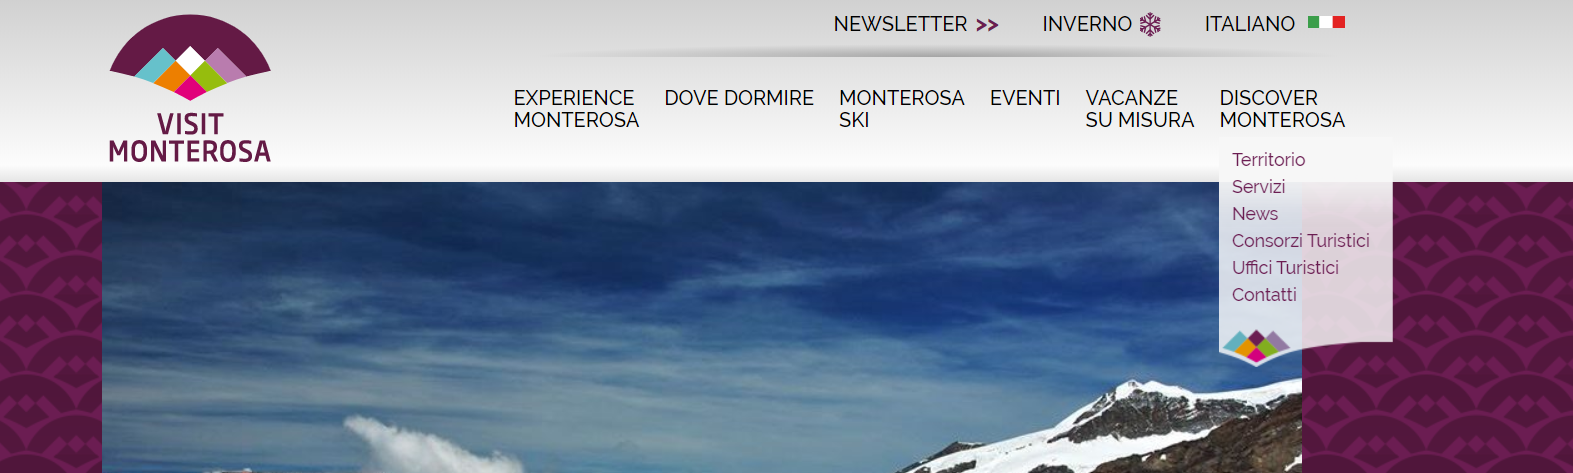
\includegraphics[scale=0.15]{resources/images/textLayout2.png}
        \end{figure}
        A causa della trasparenza il testo tende a confondersi con lo sfondo che
        presenta lo stesso colore.\\
        Il testo presenta generalmente una corretta gestione delle dimensioni che
        evidenzia una chiara distinzione delle gerarchie. Non sempre però la 
        distinzione in gerarchie è correttamente rispettata, come ad esempio:
        \begin{figure}[H] 
            \centering
            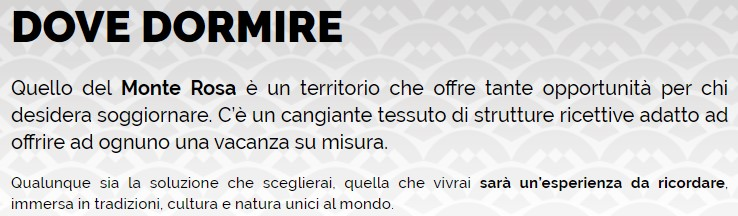
\includegraphics[scale=0.6]{resources/images/textLayout4.jpg}
        \end{figure}
        Nello screenshot riportato non c'è motivo per cui le ultime due righe
        siano più piccole delle prime.

        \subsection{Interazione dei placeholder}
        In certi casi la presenza di elementi interattivi è perfettamente
        evidente grazie all’utilizzo di colori diversi / elementi visivi
        caratterizzanti, come in questi casi:
        \begin{figure}[H]
            \centering
            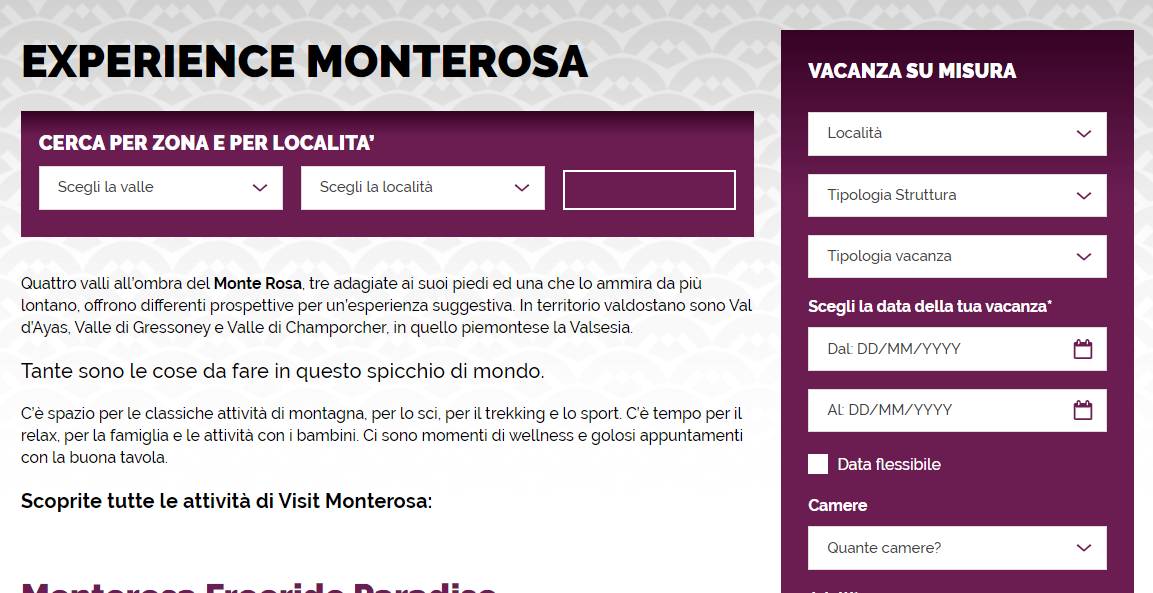
\includegraphics[scale=0.2]{resources/images/interactionPlaceholder1.png}
        \end{figure}
        In altri casi non è per nulla evidente.
        \begin{figure}[H]
            \centering 
            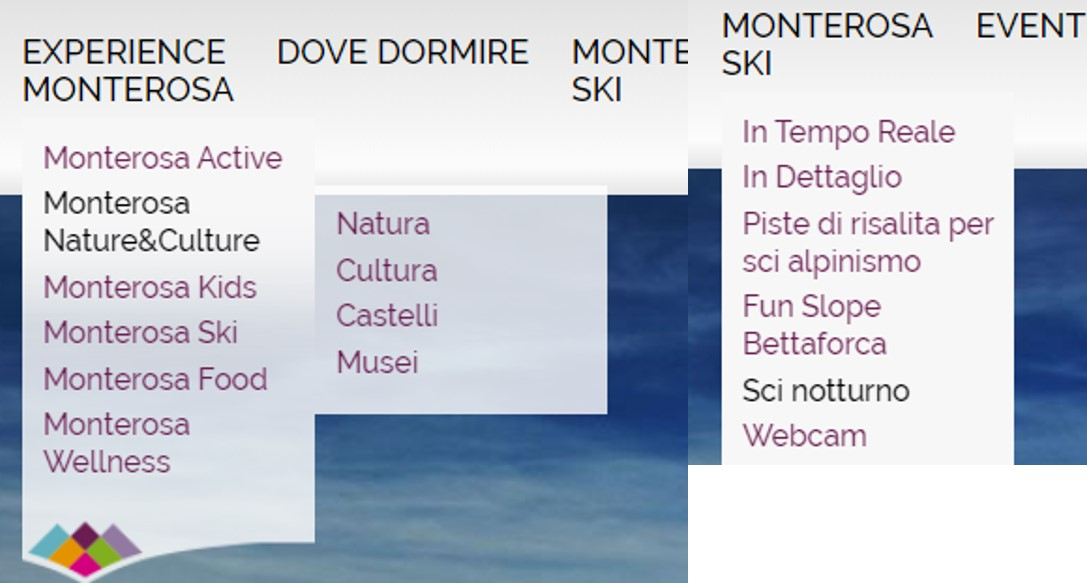
\includegraphics[scale=0.3]{resources/images/interactionPlaceholderFinal.jpg}
        \end{figure}
        Nel menu a tendina di sinistra, ad esempio, non ho nessun elemento
        visivo in grado di farmi capire che se passo il mouse sopra “Monterosa
        Nature\&Culture” si aprirà un altro menu. La scoperta di questo menu
        avviene così in maniera casuale e non so mai quale link presenta un
        sottomenu o meno (come nel caso del menu di destra). Discover Monterosa
        ed Experience Monterosa sono semanticamente simili e possono creare un
        po 'di ambiguità nella mente dell'utente riguardo a ciò che possono
        rappresentare. La presenza di un elemento Ski all'interno di Experience
        Monterosa crea ambiguità in quanto ci si aspetterebbe di trovare le
        stesse informazioni relative a quelle contenute nella pagina Monterosa
        Ski, ma così non è.
        
        \subsection{Allocazione spaziale}
        Certi elementi visivi tendono a essere dominanti su altri anche quando
        non dovrebbero esserlo. Nella pagina dedicata alle attività sul
        Monterosa ("Monterosa Active") il testo che spiega le attività è
        nascosto rispetto a tutto quello che lo circonda, quando invece dovrebbe
        essere l’elemento principale. Il menu laterale non è inoltre collegato
        semanticamente perchè la prenotazione dovrebbere essere in una pagina
        dedicata a quello. La presenza della barra laterale a sinistra inoltre è
        un elemento che riduce la Unity poichè sposta tutto a sinistra senza
        avere un corrispettivo a destra. Per quanto riguarda la Gestalt invece
        c’è una chiara divisione tra le sezioni.\\ 
        Nei landmarks tutte le informazioni relative al Monte Rosa (quindi "Monterosa
        Experience", "Monterosa Discovery" e "Monterosa Ski"), dovrebbero essere vicine 
        l'una all'altra in quanto riguardano semanticamente lo stesso argomento.\\
        Le news e le info utili inoltre dovrebbero essere vicine essendo legate
        entrambe dal fine di dare informazioni. La Barra relativa al “Cerca nel
        Sito” pur essendo utile all'utente per la ricerca risulta essere scomoda
        da trovare in quanto posizionata in basso a destra.
        \begin{figure}[H]
            \centering 
            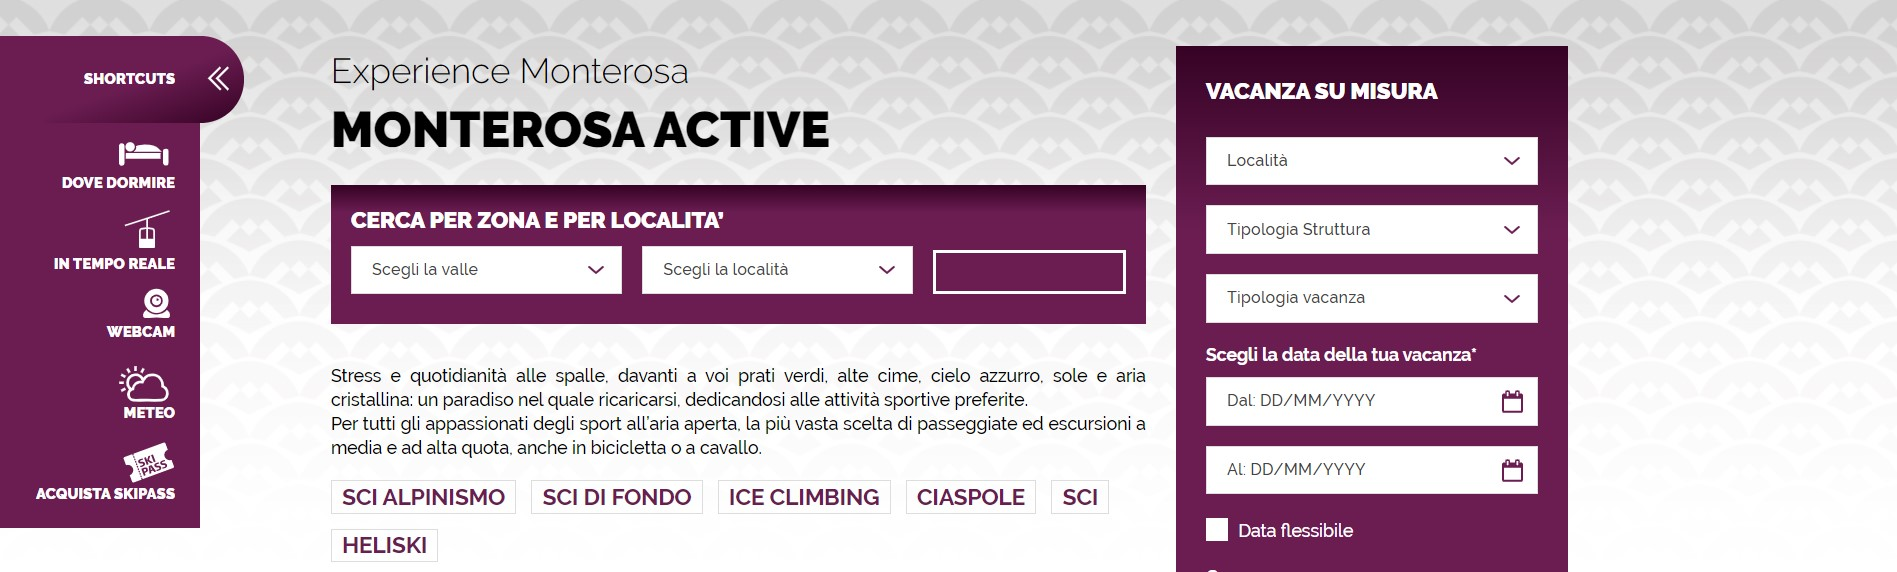
\includegraphics[scale=0.3]{resources/images/spatialAllocationFinal.jpg}
        \end{figure}
        
        \subsection{Consistenza della struttura delle pagine}
        La pagina Experience Monterosa e Discover Monterosa non hanno lo stesso
        layout anche se sono appartenenti allo stesso argomento. Un altro
        esempio sono le pagine presenti all'interno  dei link “servizi”(entrando
        da Monterosa Discovery): le sottocategorie “ristoranti e bar” e
        “shopping” appartenenti a “Visit Monterosa” hanno ad esempio layout
        differenti pur appartenendo allo stessa tipologia di pagina.